\subsection{Multiverses}
\initial{I}f you put the most vivid part of your brain in action, there are really no limits on how abstract one can make the concept of life.
Why must \textit{life} be restricted to something close to our own size?
Why must \textit{life} be restricted to something that resembles us at all?
We have mentioned the Gaia theory, but why stop there?
The Universe itself could also be considered a living organism, if what some theoretical physicists believe are true.
This is where we introduce the idea of a multiverse.

The idea goes as follows:
What if there is more than one universe?
What if these are all connected to each other in a dimension completely oblivious to us?
What if universes could create new universes?

\begin{center}
	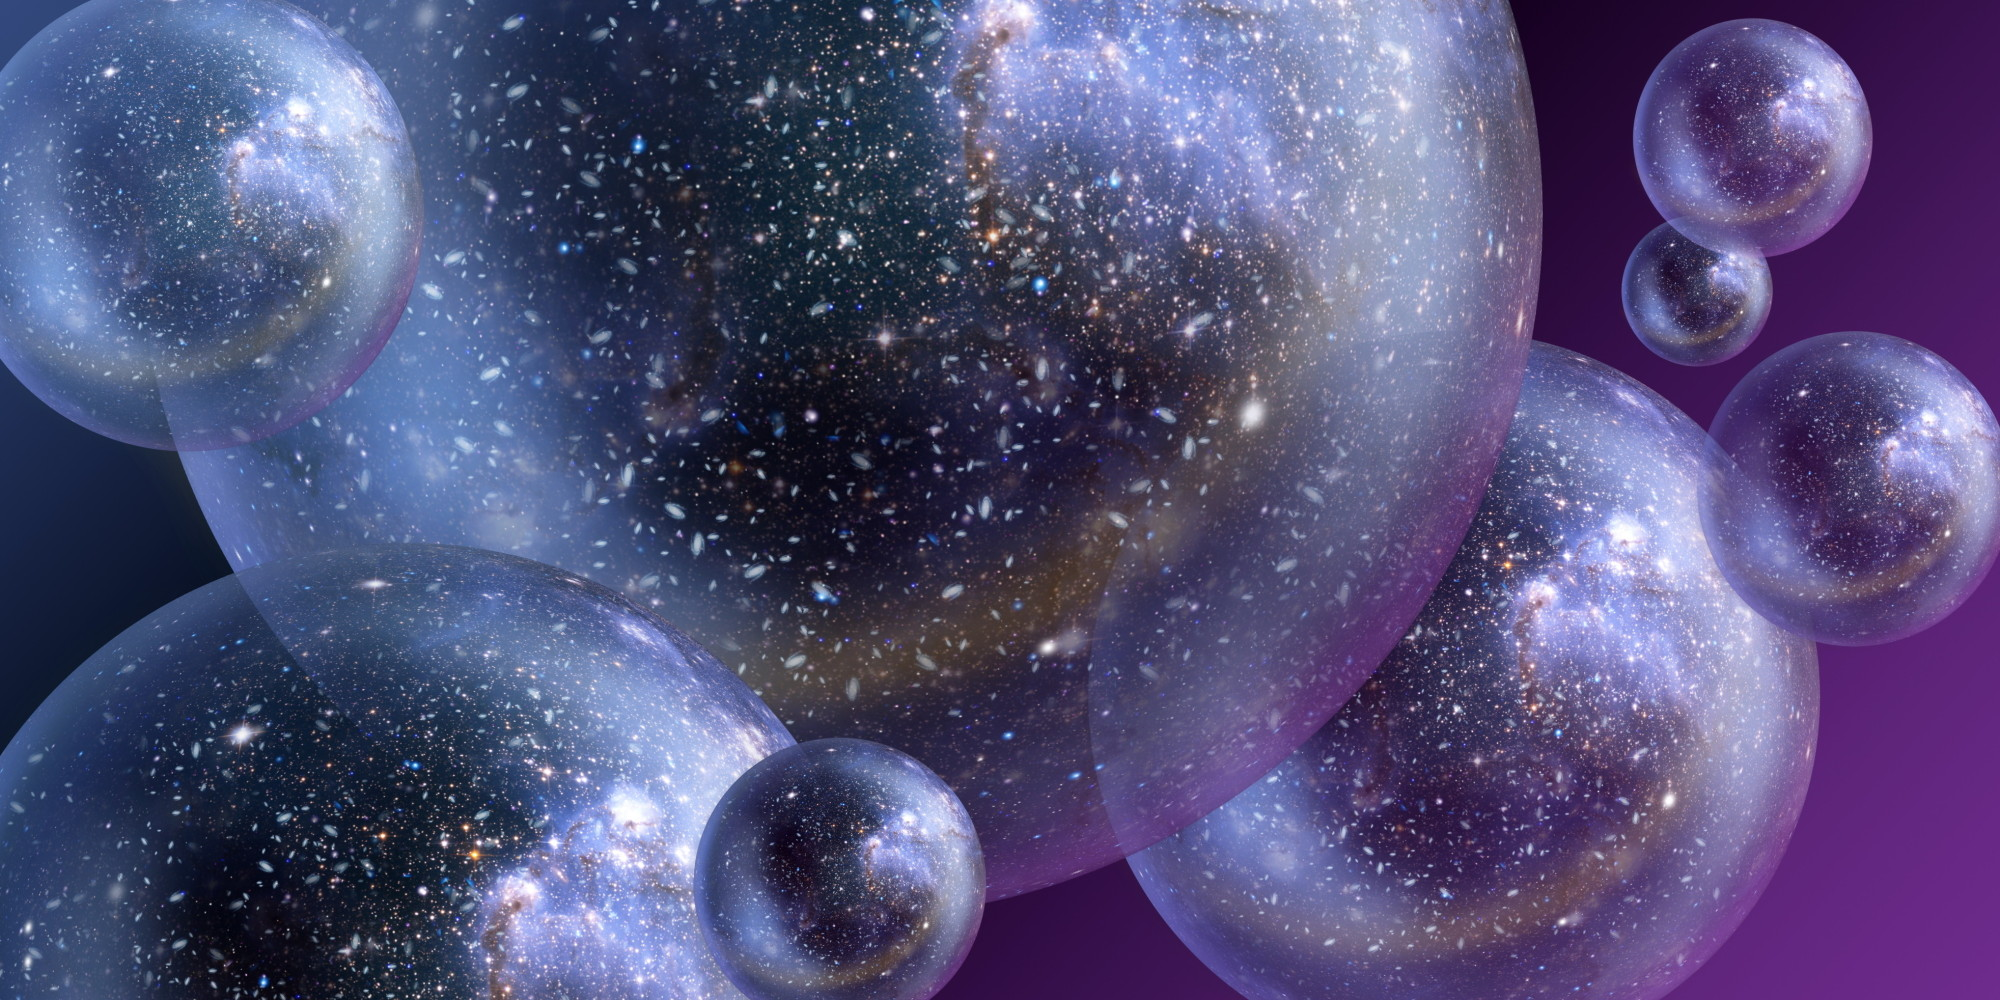
\includegraphics[width=0.475\textwidth]{multiverse.jpg}
	\tiny{Credit: Detlev van Ravenswaay}
\end{center}

Multiverse has been suggested several times in science fiction, often in context of time travel or alternate universes.
Time travel would for example, split the history into two different universes.
One where the time travel never happened and one where it did.
Alternate universes would often be a thought experiment where you could have been born in a different place and time, but still be \textit{you}.
Could there be a world out there where you are the President of the United States?

There also exists a more scientific, or less fictional, version of this idea.
In short, different universes would have different physical conditions, and all of them would pan out differently from one another.
The beginning of a universe would be something like the Big Bang.
From there it grows and changes, governed by its own physical laws and constants.
In time it may come to a stage where it creates black holes.
Some think this is how a universe might reproduce.
The newly formed universe would have slightly different attributes than its parent.
Some universes may die, some may have physical conditions that keep them in an endless cycle of expanding and retracting.

Universes could undergo birth, growth and death.
They evolve throughout their generations with every infant universe being slightly different from its parent.
Only the ones capable of creating black holes will be \textit{successful}.
How these organisms could feed and move in higher dimensions is even more vivid and far fetched.
After all, this is only an idea.
At least for now.